\chapter{Model-View-Controller for Science}\label{ch:mvcs}

\section{Introduction}\label{sec:mvc-introduction}
Developing a computer program is much more than having a few scripts that you can run when you need them. The software should take care of a lot of your concerns, such as the limits of your devices, and it should be flexible enough that it enables you to change what measurements you're performing without spending months changing the code base. More importantly, a program should be extensible in the long run, not just by you but also by future colleagues and, potentially, by anyone who finds your application online.

Therefore, when you develop software, you'll want to keep in mind the following \textbf{programmer's mantras}:

\begin{itemize}
\item What you develop should be readable by both current and future colleagues
\item It should be easy to add solutions that have been developed by others
\item The program should allow you to exchange devices that achieve the same goal (e.g., oscilloscopes of different brands)
\item The code developed in one context has to be available in other contexts (i.e., in other experiments)
\end{itemize}

Let's take a look at each of these in turn. The first mantra isn't too challenging to understand in and of itself. The second mantra talks about solutions developed by others, meaning that often another developer may have already written a driver for a device, or perhaps a measurement script. Therefore, it should be easy to get code from other developers and use their software in your projects.

The third mantra discusses exchanging hardware, which is something that's often not valued until it happens. In most labs, there's always a legacy device that sooner or later breaks down, and you'll need to replace it. In another case, you might move to a different lab and need to continue your experiments with different hardware. There are patterns that you can follow to allow a simple exchange of devices. The last mantra speaks about context. Experiments can be very different, but the logic behind them is often quite similar. You measure the I-V curve of a diode, but this is, by no means, any different from doing a 1-D scan on a confocal microscope, or tuning the wavelength of a laser.

The mantras are not rules. They're just points on which you should reflect to try and recognize when you're departing from the path you wanted to follow when you started your project. In the following sections, you're going to explore a design pattern for software that has many benefits when developing scientific software for controlling experiments. It's called \textbf{The Model-View-Controller for Science.}

\section{Understanding the MVCs Design Pattern}\label{sec:mvc}
\begin{center}
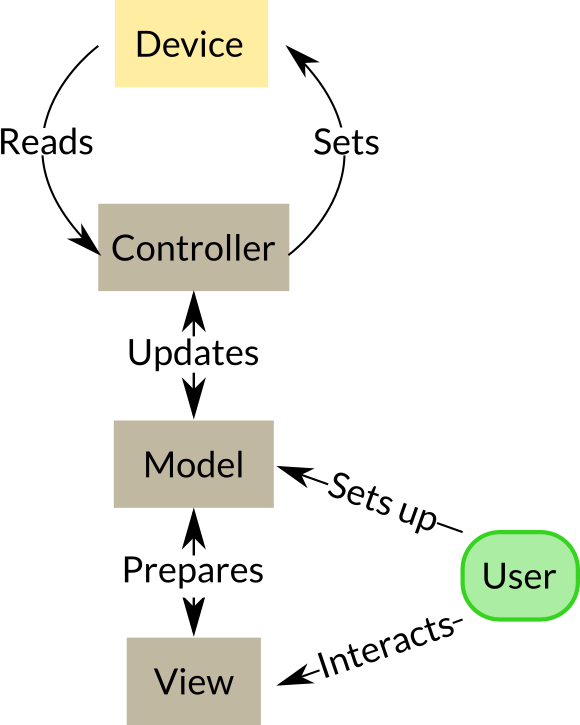
\includegraphics{images/Chapter_04/MVCs.png}
\end{center}

A \textbf{design pattern} is nothing more than a set of rules that determine where you can place different parts of the code and how they're going to interact with each other. One such pattern is called the \textbf{Model-View-Controller} pattern, or MVC for short. When you're working with devices in the lab, there's an extra layer that most computer programs lack, which is the interaction with the real world through specific devices. That's why we decided to nickname the pattern \textbf{MVCs}, with the "s" for \emph{science}. Let's take a closer look at each component of the MVC.

A \textbf{Controller} for the purposes of this book can also be called a \emph{driver}, which is responsible for communicating with devices. This can be a Python class you developed yourself, such as the one you built in the previous chapter, or it can be a Python package that was developed by someone else. For instance, many manufacturers provide drivers themselves, such as PyPylons from Basler, or the NI-DAQmx bindings for Python. The driver has to reflect the capabilities of the device, nothing more and nothing less. For example, if a device can acquire just one data point at a time, then the driver shouldn't include a function for acquiring an array of data using a loop. You saw this briefly in the previous chapter. Whatever belongs to the logic that a user imposes belongs to the Model component.

The \textbf{Model} is where all the logic is defined. This is where you determine how you're going to use a device for your experiment. A clear example would be the introduction of units. The \py{Device} class from the previous chapter takes only integer values as arguments of the methods. If you would like to transform that information into voltages, then you could do this in the model.

Moreover, in the experiment itself, you measure voltage, but you can convert it into a current with Ohm's law. This behavior is particular to your experiment, and thus the option shouldn't be hard coded in the driver. The place to include this information is the Model. The main advantage of splitting up \emph{Controllers} and \emph{Models} is that it becomes simple to upgrade or replace a device. You need to update the \emph{Model} to reflect the new options of the device, but the logic of the experiment is left intact.

There's a second type of model called the \textbf{Experiment Model} in which you link different devices to perform a measurement. You could also use a single device, but you add the features that an experiment needs (for example, saving data, plotting, analyzing, or transforming units). With straightforward cases, the boundary between the device model and the experiment model can be blurry. Still, when you're dealing with several devices or more complex workflows, it becomes much clearer. At the end of the book, we give a reference to some of the projects we've worked on, which can be a good source of inspiration.

The \emph{View} is the place where you can place everything related to how you show data to the user and how the user can change the parameters of the experiment. In practice, it's a collection of files that build up a Graphical User Interface ({GUI}). Within the {GUI}, you set, for example, the start, stop, and step of the experiment. This information is passed on to the model to acquire the data, save it, and plot it. Note, however, that the user interacts through the View with the Model, but never directly interacts with the Controller. It's also essential for you to keep in mind that all the logic is implemented in the Model. For example, if you save the data to files, the procedure to create new file names should be specified in the Model and not in the View.

For this project, the controller is what you learned about in Chapter~\ref{ch:first-driver}. The model for the device will be discussed in Chapter~\ref{ch:device-model}, the model for the experiment in Chapter~\ref{ch:experiment-model}, and the view in Chapters~\ref{ch:starting-gui} and~\ref{ch:user-input-designer}. As you can see, there are still many things to cover in the book. It's important to be patient, because you're going to grow a solution slowly, based on your needs, and solving the mistakes that may appear as you go, not just following a path blindly.

\tipsInfo{Why Separate the Code?}{For those who are new to developing code for the lab, it may be hard to understand why and how to split up the \emph{Controller} and the \emph{Model}. When you have only one device that you use for only one goal, one that is as simple as the device you're using in this book, the differences between Model and Controller are very thin. However, when you wish to include code developed by others, or when you want to share your own code, it's crucial that you separate the capabilities of your device from the logic of your experiment. If you don't do so, then all your code will only work when performing just one particular experiment.}

The meaning of \emph{Model}, \emph{View} and \emph{Controller} changes depending on each developer or community. People developing a web application are not dealing with devices in the real world, as those in the lab are. Therefore, the {MVC} pattern definition can change from one field to another. The details are not that important; once you establish a structure and follow it, then everyone else will be able to understand quickly what the code is doing and where. Once you understand what each component is, you will very quickly understand where you need to change the code to solve a bug or add new functionality.

\section{Structuring the Program}\label{sec:structure-of-theprogram}
In the program you're developing in this book, you follow the MVC design pattern quite literally. This means that you have to create three folders called \emph{Model}, \emph{View} and \emph{Controller}. In the previous chapter, you've already developed the driver for the device. Go ahead and move the file \textbf{pftl\_daq.py} into the \emph{Controller} folder.

\questionInfo{Exercise}{Create a file \textbf{analog\_daq.py} in the \emph{Model} folder. Inside the file, define a class called \mintinline{python}{AnalogDaq}. What methods do you think should belong to the device Model?}

In your definition of Model, it's vital for you to make a further distinction. On the one hand, you have models for the devices you use. In those models, you define things such as units or how to initialize the device. However, experiments often require you to perform complex tasks in which you need to synchronize several instruments. When you perform a measurement, you need to save the data or load the configuration from a file.

\questionInfo{Exercise}{Create a file in the \emph{Model} folder called \textbf{experiment.py}. Define a class called \mintinline{python}{Experiment} and add some methods that you think are going to be useful. You can, for example, add a method for switching on or off the {LED}. You can also add a method for doing a scan of an analog output signal.

The methods can be empty, so don't worry about making it work, but focus on the layout. You have to start thinking about the parameters that you need and the order in which you can call every method. For example, to save the data, you need to specify a folder first.}

The \emph{View} folder is going to require a bit more work than the other two. However, you can already start thinking about how the user is going to interact with your program. Most likely, you have thought that sometimes the {LED} will be plugged into output channel number 1, and other times to channel number 0. You don't want to change the code every time you change where you've connected the LED. The same happens, for instance, with the channel you want to monitor, or the time delay between steps. You'll include all this behavior in the View that you'll develop in the last chapters of the book.

Now that you've started to split the code into different folders and files, it's essential for you to learn how to make programs that can use the code that's located in those separate files. This process is called \textbf{importing}, and it's the focus of the next section.

\section{Importing Modules in Python}\label{sec:importing-python}
In the previous chapter, you saw some lines that look like this:

\begin{minted}{python}
import numpy as np
from time import sleep
\end{minted}

The first line imports the NumPy package, but changes its name to \mintinline{python}{np}. Changing the name makes it easier for you to work with libraries, since you can type fewer letters (\mintinline{python}{np} instead of \mintinline{python}{numpy}). The second line is importing one specific function from a package called \mintinline{python}{time}. It's important for you to realize that the import process is different in both cases. NumPy is a complex package, with many modules that you can use. The same is true for \emph{time}. However, in the lines above, you have only imported the module \emph{sleep} from the package \emph{time}. If you want to use it, you can do this:

\begin{minted}{python}
sleep(1)
\end{minted}

With \emph{Numpy}, you will need to specify which module you want:

\begin{minted}{python}
np.random.random(1)
\end{minted}

If you know you only want to use \mintinline{python}{random} from NumPy, then you can also import and use it like this:

\begin{minted}{python}
from numpy.random import random

random(1)
\end{minted}

You may wonder why you would import all of NumPy if you're just using one of its functions. Well, the name \emph{random} is not defined solely by NumPy. Python also provides its own \py{random} module. You can import it like this:

\begin{minted}{python}
import random
\end{minted}

If you needed both \emph{random} functions (the one from NumPy and the one from Python's standard library) in the same program, you would have a clash. How could you be sure that you're using NumPy's function and not Python's? What's more, you might even define your own random function, and you would like to be able to choose which one to use. More importantly, you want to avoid generating unexpected behavior because of redefining functions without realizing it.

When working with your code, you can import different modules in the same way. Open a terminal and navigate to the root folder of the project. This is the folder that contains the \emph{Model}, \emph{View}, and \emph{Controller} folders. Start the Python interpreter, and then type this:

\begin{minted}{pycon}
>>> from Controller.pftl_daq import Device
\end{minted}

Now you have the controller available for use. You can then do the following:

\begin{minted}{pycon}
>>> dev = Device('/dev/ttyACM0')
>>> dev.initialize()
\end{minted}

However, something strange happens if you run the code above. As soon as you import \py{Device}, the program starts communicating with the device, outputs the identification number, and switches on and off the LED. This behavior is something you don't want, and this is a very common pitfall for Python developers. Of course, you don't want the code to trigger a measurement just because you imported the module into your program.

To avoid having the code run as soon as an import happens, you must change the file \textbf{pftl\_daq.py}. You can add one line of code at the end of the file, as well as some indentation, to make it look like this:

\begin{minted}{python}
if __name__ == "__main__":
    dev = Device('/dev/ttyACM0') #<---- Remember to change the port
    dev.initialize()
    serial_number = dev.idn()
    print(f'The device serial number is: {serial_number}')
    for i in range(10):
        dev.set_analog_output(0, 4000)
        volts = dev.get_analog_input(0)
        print(f'Measured {volts}')
        sleep(.5)
        dev.set_analog_output(0, 0)
        volts = dev.get_analog_input(0)
        print(f'Measured {volts}')
        sleep(.5)
\end{minted}

To see the changes, you first must close Python by running the \py{exit()} command and then open it again. Python won't import the same modules twice, so it won't realize that the file with your Controller changed. After you restart Python, you can try to import the Controller again. Now, things are going to look fine, and you can use the \py{Device} as you intended. You can leave the space at the bottom of the files to hold examples of how to use the code above. If you ever find the Device around, and you don't remember what you were supposed to do with it, you can always go to the bottom of the file and see how it works.

Every time you encounter a behavior that's not easy to understand, the best idea is for you to transform it into simpler components and explore them one by one. In this case, the import process may be a bit confusing. To understand it a bit more, especially with respect to how the line \mintinline{python}{if __name__} works, you can create a new file called \textbf{dummy\_controller.py} in the \emph{Controller} folder with the following lines of code:

\begin{minted}{python}
print('This is the dummy Controller')

def dummy_example():
    print('This is a function in the dummy Controller')

if __name__ == '__main__':
    print('This is printed only from __main__')
    dummy_example()

\end{minted}

\sloppy From the Terminal, you can just type \py{python Controller.dummy_controller.py}. The output should be like what you see below:

\begin{minted}{bash}
This is the dummy Controller
This is printed only from __main__
This is a function in the dummy Controller
\end{minted}

What you see is that the entire code was executed.

\questionInfo{Exercise}{What do you expect to happen if you run \mintinline{python}{import dummy_controller}?}

Things are going to be different when you import the file. In the Python interpreter you can do the following:

\begin{minted}{pycon}
>>> from Controller import dummy_controller
This is the dummy Controller
>>> dummy_controller.dummy_example()
This is a function in the dummy Controller
>>> from Controller.dummy_controller import dummy_example
>>> dummy_example()
This is a function in the dummy Controller
\end{minted}

First, notice that the code at the end never gets executed. This means that the \py{if} statement is not \py{True}. This block is handy when you want to have code that works as a standalone (when you execute it directly, for example), but you don't want to execute those lines if you import. In the case of the real Controller, we wanted to leave some examples at the end to show how you can use it, but when you're importing a class, you don't want it to start communicating with the device.

\sloppy You can also see that the line \py{"This is the dummy Controller"} appears only once. Python knows that you've already imported the module \textbf{dummy\_controller}, and it won't execute those import lines again. Therefore, you have to be aware that it's not a matter of using the \py{from} in the importing procedure. You can close Python, start it again and revert the order in which you import, and the print will still be there the first time but not the second. It means that Python is smart when importing modules, and it won't fetch the elements it already has available, even if you're importing in a slightly different way.

\tipsInfo{Naming Conventions}{We should establish some naming conventions to avoid confusion later on. In Python, any file that defines variables, functions, or classes is called a \mintinline{python}{Module}. The folder that contains modules is called a \mintinline{python}{Package}.}

Python imports might be easier to work with than they are to understand, especially when you're trying to pay attention to all the different definitions. The Official Python Documentation\footnote{https://docs.python.org/3.6/tutorial/modules.html} has an excellent chapter covering a lot of the ideas discussed. Many of the properties and behaviors can be learned through trial and error, though this can be very time consuming, and it may lead to unexpected errors.

There's one final remark that's worth mentioning about packages. Right now, you have three folders in your project: \emph{Model}, \emph{View}, and \emph{Controller}. But what would happen if you added a new folder called, for example, \emph{serial}? Next time you try to \py{import serial}, how would Python know whether it's supposed to import the PySerial library or your package? This can also happen the other way around. Perhaps you don't know that there's something already called \emph{Controller} in Python, and you don't care about this module; you want to import your own modules.

For Python to understand that a folder is a \emph{package}, you should add an empty file to the folder called \textbf{\_\_init\_\_.py}. This file is the way of letting Python know that a folder is more than just a plain directory, and thus it should be treated accordingly. In other words, you must add the empty init files in the three folders you have created so far. If you're using a Python IDE, such as PyCharm, notice that these files are created automatically if you chose 'new package' while trying to add a folder.

\questionInfo{Exercise}{Create a folder called \emph{random} and inside of that create a new file called \textbf{test.py}. Define a function inside the file. It's not important what it does. Then, save it. Start Python and see what happens if you run \mintinline{python}{from random import test}. Quit the interpreter and add an empty file called \textbf{\_\_init.py\_\_} inside the \textbf{random} folder. Try to import \py{test} again and see what happens.}

The init files of packages allow you to specify more complex behaviors when importing, but that goes beyond the scope of this book. Going through other packages is an excellent way of understanding how developers have decided to structure their code.

\section{Changing the PATH Variable}\label{sec:path}
There's still a huge difference in the way you perform imports when you compare your own code to a library such as NumPy. Packages like NumPy can be imported regardless of where you've started the Python interpreter. You can go to any folder in the Terminal, start Python, and \py{import numpy}. However, you can only import your package if you're in its directory. If you're sitting in a different folder and try to import the Controller, you get an error like the following:

\begin{minted}{pycon}
>>> from Controller.pftl_daq import Device
Traceback (most recent call last):
  File "<stdin>", line 1, in <module>
ModuleNotFoundError: No module named 'controller'
\end{minted}

Python searches for packages in specific locations, and once it finds one, it stops searching. NumPy is located in one of the folders that Python searches, but Python is not aware of your package yet. One way to let Python know where your package is located is to add the folder to a system variable called \mintinline{bash}{PYTHONPATH}.

On Windows, you can follow the steps explained in Section~\ref{subsec:path-windows}, where you were dealing with the details of adding environment variables after installing Python. The only difference is that you should use the variable \mintinline{bash}{PYTHONPATH} instead of just \mintinline{bash}{PATH}. On Linux, it's enough to run the following command:

\begin{minted}{bash}
$ export PYTHONPATH=$PYTHONPATH":/path/to/PFTL"
\end{minted}

You have to replace \py{/path/to/PFTL} with the full path to the folder where you're keeping the code. After running that, you can type \py{from Controller import *} wherever you are in your computer, and Python will find the appropriate folder. On Linux, this change is not permanent, so you'll need to rerun the command the next time you start the Terminal. You can modify environment variables permanently, but that goes too much into the details of the operating systems. We leave this as an exercise for the reader.

If you're using an IDE to develop and run the code, you may have noticed that there's no need to add anything to the Python path. This is one of the advantages of using robust programs to develop software. They take care of many things for you. However, at some point, it's also essential for you to be able to run the program independently of the editor software.

\section{Finalizing the Layout}\label{sec:final-layout}
At this stage, you should have a clear separation of the code into folders titled \emph{Model}, \emph{Controller}, and \emph{View}. Most of these are, for the time being, empty folders. However, you're not limited to having only three folders in your project. Most likely, you want to provide some examples of how to use the code or some documentation.

However, if you create extra folders next to the three main ones, then the structure of the program will start to become polluted. It won't be clear what's part of the program and what's a user-specific setting. Therefore, it's a common practice to make a folder to hold the program itself. Then, next to it, you create an extra folder to contain any non-essential elements. In this case, the folder structure could look like this:

\begin{minted}{text}
├── Docs/
├── Examples/
└── PythonForTheLab/
    ├── Controller/
    │   ├── __init__.py
    │   └── pftl_daq_01.py
    ├── Model/
    │   └── __init__.py
    ├── View/
    │   └── __init__.py
    └── __init__.py
\end{minted}

There are three folders at the top level: \emph{Docs}, \emph{Examples}, and \emph{PythonForTheLab}. This last folder holds the \emph{Model}, \emph{View} and \emph{Controller} folders with all the code that you've developed up until now. The folder \emph{PythonForTheLab} also requires an \textbf{\_\_init\_\_.py} file, because it's your main package. This folder structure would allow you to do the following:

\begin{minted}{pycon}
>>> from PythonForTheLab.Controller import pftl_daq
\end{minted}

This code is cleaner than importing the Controller directly because it also allows you to, in principle, have different programs at the same time and import only the elements you need from each one. For example, you could have one big project with many devices and complex measurements, and a smaller program to do more specialized tasks that only require some of those devices.

\section{Conclusions}\label{sec:layout-conclusions}
Following a pattern when you're programming makes your code much easier to understand, maintain, and explain to others. Patterns, however, are not set in stone. Sometimes there's no clear divide between what you should develop and where you should put it. The important thing is for you to be consistent. For example, if at some point it's decided that controllers should handle real-world units, then all controllers should do so. If, on the other hand, you decide that models should handle units, then all models should do so, regardless of what the specific controllers do.

Following a pattern is useful not only when there are many developers involved in the same project, but also when the same person is working on different projects, or if a person were to change labs or experiments. As time passes, you start accumulating a collection of tools, and being able to transfer them from one experiment to another makes it much faster for you to have a measurement running without reinventing the wheel over and over again.

Another essential aspect for many scientists is that solutions should be developed as quickly as possible to test out new ideas, and this is how we laid out this book. First, you manage to quickly communicate with the device. You saw that you can acquire data and switch the LED on and off. If the measurement was a one-off task, then you would be finished. However, if you'd like to start changing parameters, or if you want to use the code for another experiment, then you need to keep going. Expanding the code is what you're going to do next. In these sections, you have explored a sustainable way of following the \emph{Onion Principle}. Factoring also tackles concerns about the speed at which you can implement a solution for the lab.

The strategies proposed in this chapter do not come naturally to every developer, and even if you know them, you can try to find shortcuts. The truth is that no one does an experiment only once. The key to better science is reproducibility, and the clearer the code that enabled you to acquire data, the easier it is to repeat a measurement, even for someone else. We can only lay out the foundations for what we consider a robust solution. If you find a different path, you're always free to follow it, but never forget the bigger picture.
